\documentclass[11pt,a4paper]{article}

% Packages
\usepackage[margin=1in]{geometry}
\usepackage{amsmath,amssymb,amsfonts}
\usepackage{graphicx}
\usepackage{booktabs}
\usepackage{hyperref}
\usepackage{xcolor}
\usepackage{listings}
\usepackage{enumitem}
\usepackage{caption}
\usepackage{float}
\usepackage{fancyhdr}
\usepackage{titlesec}

% Colors
\definecolor{codegreen}{rgb}{0,0.5,0}
\definecolor{codegray}{rgb}{0.5,0.5,0.5}
\definecolor{codebg}{rgb}{0.96,0.96,0.96}
\definecolor{accentblue}{rgb}{0.1,0.3,0.6}

% Listings style
\lstset{
    basicstyle=\ttfamily\small,
    backgroundcolor=\color{codebg},
    keywordstyle=\color{accentblue}\bfseries,
    commentstyle=\color{codegreen},
    stringstyle=\color{red!60!black},
    numbers=left,
    numberstyle=\tiny\color{codegray},
    numbersep=5pt,
    frame=single,
    breaklines=true,
    captionpos=b,
    language=Python,
}

% Header
\pagestyle{fancy}
\fancyhf{}
\fancyhead[L]{\small COSC 739 -- Extension 1: Generative Canary Ensemble}
\fancyhead[R]{\small Al-Jallad \& Thabet}
\fancyfoot[C]{\thepage}

% Section formatting
\titleformat{\section}{\Large\bfseries\color{accentblue}}{\thesection}{1em}{}
\titleformat{\subsection}{\large\bfseries\color{accentblue!80}}{\thesubsection}{1em}{}

\begin{document}

% ============================================================
% Title
% ============================================================
\begin{center}
    {\LARGE\bfseries Extension 1: Generative Canary Ensemble\\[6pt]
    \large Scaling Defensive Patch Diversity for Adaptive Attack Resistance}\\[12pt]
    {\large Leen Al-Jallad (100067697) \quad Mohamed Thabet (100066980)}\\[4pt]
    {\normalsize Department of Computer Science, Khalifa University}\\
    {\normalsize COSC 739 -- Security of Machine Learning Systems}\\[6pt]
    {\normalsize April 2026}
\end{center}

\vspace{0.5cm}
\hrule
\vspace{0.5cm}

% ============================================================
\section{Original Paper Summary}
% ============================================================

The ``Fight Fire with Fire'' (FFF) framework by Feng et al.\ (IEEE S\&P 2025) proposes a defense against adversarial patch attacks on object detectors. Adversarial patches are physically printable patterns that, when worn by a person, suppress their detection by models such as YOLOv8. The FFF framework counters this by inserting specially crafted \textit{defensive patches} into the input image without modifying the underlying detector.

Two types of defensive patches are introduced. The \textbf{canary} is a fragile recognizable object (e.g., a zebra image, 80$\times$80 pixels) placed near bounding boxes that the detector identifies as potentially suppressed. If the detector fails to recognize the canary, adversarial interference is suspected. The \textbf{woodpecker} attempts to restore suppressed detections; if a person reappears after insertion, the attack is confirmed.

The framework operates in three deployment modes: Mode \#1 (canary alone), Mode \#2 (woodpecker alone), and Mode \#3 (combined). The key advantage is that the target detector remains completely unmodified---only the input image is augmented. On the VOC07 dataset with YOLOv8, the paper reports F1 scores up to 0.974 with false positive rates around 4.9\%.

The canary training loss is defined as:
\begin{equation}
    \mathcal{L}_{\text{Canary}} = \lambda_c \mathcal{L}_{\text{benign}} - \mathcal{L}_{\text{adv}}
\end{equation}
where $\mathcal{L}_{\text{benign}}$ encourages the canary to be detected on clean images, and $\mathcal{L}_{\text{adv}}$ corresponds to the detection loss on adversarial images. The weights are set to $\lambda_c = 2.0$. Both losses consist of objectness loss $\mathcal{L}_o$, class confidence loss $\mathcal{L}_c$, and bounding box loss $\mathcal{L}_b$. Only the canary pixel values are optimized---YOLOv8 remains frozen throughout training.

To resist adaptive attackers, the paper proposes randomized deployment: multiple canary classes (e.g., zebra, elephant, giraffe) and multiple placement positions are combined. At inference time, a random canary is placed at a random position. The paper evaluates this with $K=3$ canary types and 2 positions (6 combinations total), reporting that adaptive attacks could not bypass the defense even after extended optimization.

% ============================================================
\section{The Gap: Hardware-Dependent Security}
% ============================================================

The original paper's primary security claim against adaptive attacks is empirical: it took \textbf{37 days on an RTX 3090} GPU to attempt adaptive attacks against the randomized canary defense (Table 9, Dep \#2), and none of the 488 test samples were successfully bypassed.

However, this 37-day figure is a \textit{wall-clock measurement}, not a complexity bound. The original paper does not provide a detailed breakdown of per-iteration cost, convergence criteria, or learning rate schedules for the adaptive attack. The security guarantee is therefore tied to the specific hardware used.

Modern GPUs are substantially faster. The RTX 3090 delivers 71 TFLOPS at FP16. Current-generation GPUs offer dramatically higher throughput:

\begin{table}[H]
\centering
\caption{GPU comparison and projected time to break the fixed canary defense (3 canaries $\times$ 2 positions = 6 terms).}
\begin{tabular}{lrrr}
\toprule
\textbf{GPU} & \textbf{FP16 TFLOPS} & \textbf{Speedup vs 3090} & \textbf{Projected Time} \\
\midrule
RTX 3090 & 71 & 1$\times$ & 37 days \\
B100 & 1,750 & $\sim$25$\times$ & $\sim$1.5 days \\
B200 & 2,250 & $\sim$32$\times$ & $\sim$1.2 days \\
8$\times$ B200 & 18,000 & $\sim$253$\times$ & $\sim$3.5 hours \\
\bottomrule
\end{tabular}
\label{tab:gpu_comparison}
\end{table}

The implication is clear: the fixed canary pool's security degrades linearly with hardware improvements. An attacker with access to a single B200 GPU---commercially available today---can break the defense in approximately 1.2 days. A cluster of 8 B200s could accomplish this in hours.

The fundamental issue is that the fixed pool contains a finite, enumerable set of canaries. The attacker's optimization problem is a finite sum:
\begin{equation}
    \delta^* = \arg\min_\delta \sum_{k=1}^{K} \left[ \mathcal{L}_{\text{AdvPatch}}(x + \delta) + \mathcal{L}_{\text{adv}}(c_{x+\delta}^k) \right]
\end{equation}
where $K=6$ (3 canary types $\times$ 2 positions). This is a tractable optimization with full gradient access to every term. More compute power directly translates to faster solutions---the problem size never changes.

% ============================================================
\section{Our Proposed Solution: Generative Canary}
% ============================================================

We propose replacing the fixed canary pool with a \textbf{learned generator} that produces unique canary patches at inference time. Instead of selecting from a pre-trained set, a lightweight neural network $G_\theta(z, b)$ generates a fresh canary for every image processed.

\subsection{Architecture}

The generator takes a combined input vector:
\begin{equation}
    z = [\eta \| b] \in \mathbb{R}^{132}, \quad \eta \sim \mathcal{N}(0, I_{128}), \quad b = (x_1, y_1, x_2, y_2)_{\text{norm}}
\end{equation}
where $\eta$ is a 128-dimensional random noise vector and $b$ contains normalized bounding box coordinates providing scene context.

The forward pass consists of fully connected layers followed by transposed convolutions:

\begin{lstlisting}[caption={GenerativeCanary architecture ($\sim$693K parameters).}]
class GenerativeCanary(nn.Module):
    def __init__(self, z_dim=128, bbox_dim=4, canary_size=80):
        super().__init__()
        input_dim = z_dim + bbox_dim  # 132

        self.fc = nn.Sequential(
            nn.Linear(input_dim, 256), nn.ReLU(),
            nn.Linear(256, 512),      nn.ReLU(),
            nn.Linear(512, 1024),     nn.ReLU(),
        )
        self.deconv = nn.Sequential(
            nn.ConvTranspose2d(16, 8, kernel_size=4,
                               stride=2, padding=1),
            nn.ReLU(),
            nn.ConvTranspose2d(8, 3, kernel_size=4,
                               stride=2, padding=1),
            nn.Sigmoid(),
        )

    def forward(self, z):
        x = self.fc(z)             # (batch, 1024)
        x = x.view(-1, 16, 8, 8)  # (batch, 16, 8, 8)
        x = self.deconv(x)         # (batch, 3, 32, 32)
        x = F.interpolate(x, size=(80, 80),
                          mode='bilinear')
        return x  # (batch, 3, 80, 80), pixels in [0,1]
\end{lstlisting}

\subsection{Training Objective}

The generator replaces the fixed canary in the FFF pipeline. Instead of optimizing pixel values of a static image, we optimize the generator weights $\theta$:
\begin{equation}
    \min_\theta \; \lambda_c \mathcal{L}_{\text{canary}}(G_\theta) + \lambda_w \mathcal{L}_{\text{wood}}
\end{equation}

Gradients flow from the detection loss through the frozen YOLOv8 detector, through the generated canary pixels, and back into the generator weights. At each training step, a fresh $z$ is sampled, producing a different canary that must satisfy the FFF loss. After training, the generator has learned a \textit{recipe} for producing functional canaries---not just one specific canary.

\subsection{Inference}

At inference time, the trained generator (frozen, no further training) receives a fresh random $z$ for each input image. A single forward pass ($\sim$5 milliseconds) produces a unique canary. The attacker cannot predict which canary will appear because the noise $\eta$ is sampled at runtime.

% ============================================================
\section{What We Tried and What Failed}
% ============================================================

Training a single generator to produce diverse canaries proved challenging due to \textbf{mode collapse}---the phenomenon where the generator learns to produce essentially the same output regardless of the input noise.

\subsection{Mode Collapse in the Single Generator}

Our initial single-generator experiments produced canaries that were functionally effective (F1 0.901--0.922, near-perfect recall) but visually near-identical. Quantitative measurements confirmed the collapse: pairwise cosine similarity of 0.9957 (99.6\% identical) and L2 distance of only 5.40 across 8 generated canaries.

The root cause is that the detection loss creates one strong attractor in the output space. The generator discovers a single pattern that maximizes detectability by YOLOv8 and produces that pattern regardless of the input noise. The 128-dimensional noise vector is effectively ignored.

\begin{figure}[H]
\centering
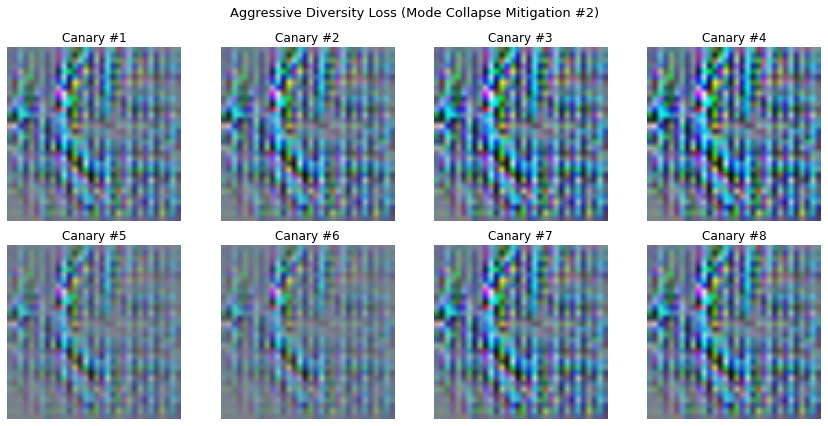
\includegraphics[width=0.85\textwidth]{figs/fig2.png}
\caption{Mode collapse: 8 canaries generated with different $z$ vectors from a single trained generator. Despite different inputs, the outputs are nearly identical (cosine similarity = 0.9957, mean pairwise L2 = 5.40). Even with an aggressive diversity loss ($\lambda_{\text{div}}=50$), the detection-loss attractor dominates and all 8 samples collapse to the same striped pattern.}
\label{fig:mode_collapse}
\end{figure}

\subsection{Approach 1: Multi-Class Conditioning (Failed)}

We extended the generator to accept a one-hot class ID alongside the noise and bbox inputs, conditioning on 6 COCO classes (horse, sheep, cow, elephant, zebra, giraffe). The hypothesis was that different target classes would force structurally different outputs.

The result: \textbf{training diverged}. Benign loss climbed from 74.45 to 125.57 (should decrease), while adversarial loss dropped from 87.01 to 69.98 (should stay high). The 6-dimensional one-hot class signal was too weak relative to the 128-dimensional noise and 4-dimensional bbox inputs---the generator ignored the class conditioning entirely. All canaries across all 6 classes looked identical.

\begin{figure}[H]
\centering
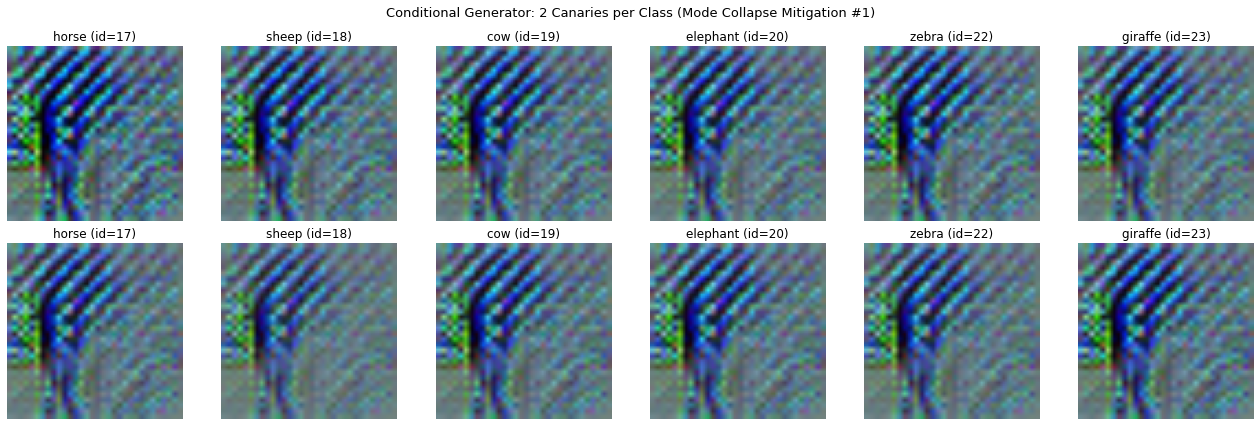
\includegraphics[width=\textwidth]{figs/fig1.png}
\caption{Approach 1 failure: 2 canaries per class across 6 COCO target classes (horse, sheep, cow, elephant, zebra, giraffe). Despite the class conditioning, every output is visually identical---the generator treats the class one-hot as noise and collapses to a single mode regardless of the target class.}
\label{fig:approach1_fail}
\end{figure}

\subsection{Approach 2: Aggressive Diversity Loss (Failed)}

We added a cosine diversity loss to the training objective, penalizing the generator when batch members produced similar outputs:
\begin{equation}
    \mathcal{L}_{\text{total}} = \lambda_c \mathcal{L}_{\text{benign}} - \mathcal{L}_{\text{adv}} + \lambda_{\text{div}} \mathcal{L}_{\text{diversity}}
\end{equation}
where $\mathcal{L}_{\text{diversity}}$ maximizes pairwise (1 - cosine similarity) across the batch. We set $\lambda_{\text{div}} = 50.0$.

The result: \textbf{no meaningful improvement}. Cosine similarity remained at 0.9957, L2 distance at 5.40. The detection loss attractor was simply too strong for the diversity penalty to overcome. Increasing $\lambda_{\text{div}}$ further risked the same training divergence observed in Approach 1.

\subsection{Key Insight}

These failures revealed a fundamental property of the problem: \textit{a single generator inherently wants to collapse}. The detection loss creates a single optimal mode that dominates any diversity-encouraging signals. The solution must sidestep the loss landscape entirely rather than fight it.

% ============================================================
\section{What Worked: Ensemble of Generators}
% ============================================================

\subsection{Approach 3: Independent Ensemble}

Instead of forcing one generator to produce diverse outputs, we train \textbf{multiple independent generators} with different random seeds. Each generator independently mode-collapses, but because of different weight initializations and training trajectories, they collapse to \textit{different modes}.

The training procedure is identical for each generator---only the random seed changes. This is conceptually similar to how different random initializations in neural network training lead to different local minima.

\subsection{5-Generator Proof of Concept}

We trained 5 generators with seeds 301--305, each for 50 epochs. Training took approximately 3.4 minutes per generator on an RTX 3070 Ti.

\begin{figure}[H]
\centering
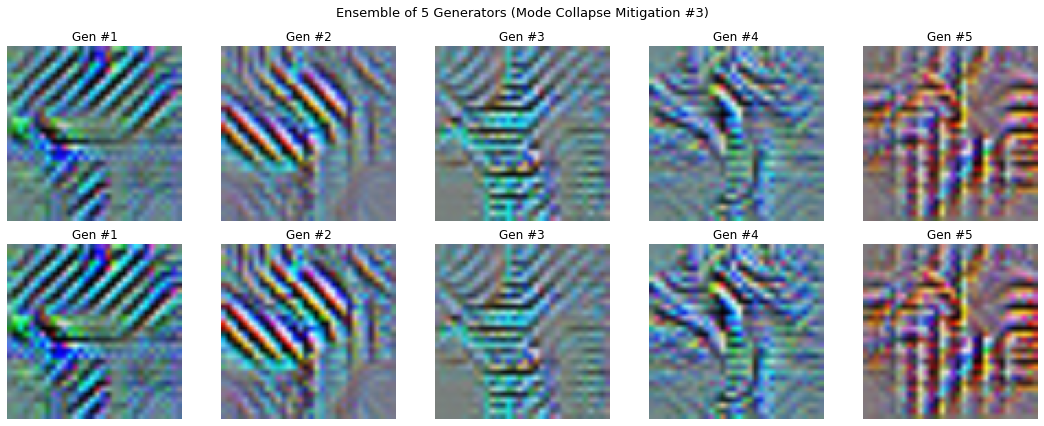
\includegraphics[width=0.85\textwidth]{figs/fig3.png}
\caption{Ensemble of 5 generators: each generator collapses to a different mode (columns), providing inter-generator diversity. Within-generator samples (rows) are similar, but across generators the patterns are clearly distinct---different stripe orientations, color palettes, and textures.}
\label{fig:ensemble_5}
\end{figure}

The diversity metrics confirmed the approach:

\begin{table}[H]
\centering
\caption{Diversity comparison: single generator vs.\ 5-generator ensemble.}
\begin{tabular}{lrr}
\toprule
\textbf{Metric} & \textbf{Single Generator} & \textbf{5-Gen Ensemble} \\
\midrule
Mean pairwise L2 distance & 5.40 & 29.56 \\
Cosine similarity & 0.9957 & --- \\
Improvement factor & 1$\times$ & 5.5$\times$ \\
\bottomrule
\end{tabular}
\end{table}

Evaluation on VOC07 showed the ensemble was functional: F1 scores of 0.935 (AdvPatch), 0.908 (UPC), 0.905 (TCEGA), and 0.929 (Natural), with FPR in the range 0.102--0.158.

% ============================================================
\section{Scaling to 1000 Generators on HPC}
% ============================================================

To make adaptive attacks computationally infeasible rather than merely inconvenient, we scaled the ensemble from 5 to 1000 generators using high-performance computing.

\subsection{Infrastructure}

We used a cloud HPC instance with 4$\times$ NVIDIA T4 GPUs (16 GB VRAM each, 65 TFLOPS FP16, \$2.75/hour total). A multi-GPU parallel training script distributed the workload evenly:

\begin{lstlisting}[caption={Parallel training: 4 workers, 250 generators each.}]
# Worker GPU 0: generators [0, 250)
# Worker GPU 1: generators [250, 500)
# Worker GPU 2: generators [500, 750)
# Worker GPU 3: generators [750, 1000)

# Each worker:
# 1. Loads YOLOv8 detector (frozen)
# 2. Preloads 120 training images into RAM
# 3. Trains 250 generators sequentially
# 4. Saves checkpoints to shared directory
\end{lstlisting}

Each generator used a unique seed (seed = generator index + 1), ensuring different weight initializations and training trajectories.

\subsection{Training Results}

\begin{table}[H]
\centering
\caption{HPC training summary.}
\begin{tabular}{lr}
\toprule
\textbf{Parameter} & \textbf{Value} \\
\midrule
Number of generators & 1,000 \\
Epochs per generator & 50 \\
Time per generator & $\sim$3.4 minutes \\
Total wall-clock time & 18.04 hours \\
GPUs used & 4$\times$ T4 \\
Total cost & $\sim$\$16 \\
Checkpoint size (each) & 2.64 MB \\
Total checkpoint storage & 2.58 GB \\
\bottomrule
\end{tabular}
\end{table}

The training script included full resume support---if interrupted, restarting would skip all completed generators and continue from where it left off. All 1,000 generators completed successfully with 0 skipped.

\begin{figure}[H]
\centering
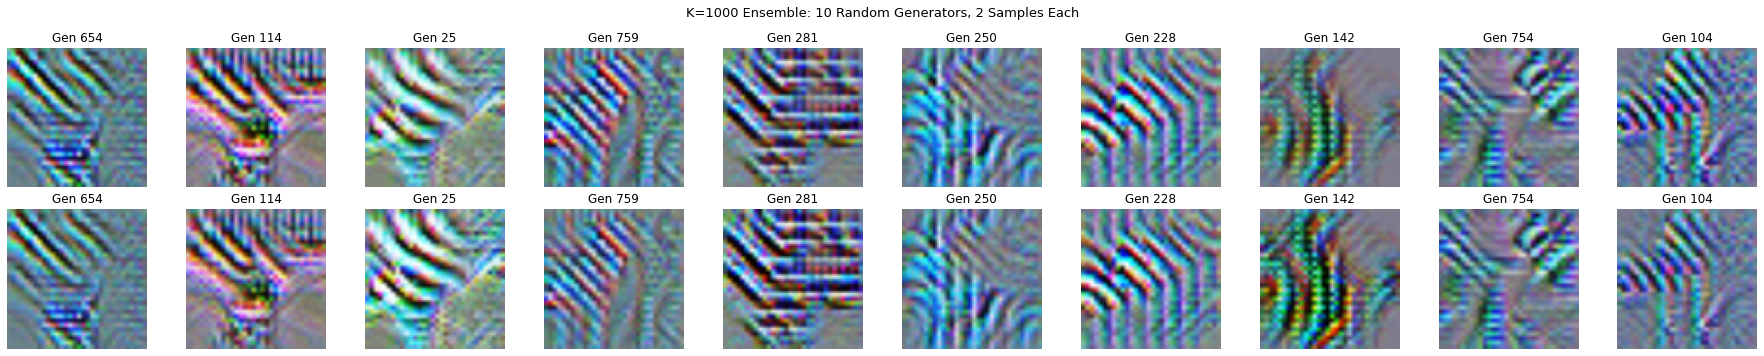
\includegraphics[width=\textwidth]{figs/fig4.png}
\caption{Quick-look snapshot of the 1000-generator ensemble: 2 samples from each of 10 randomly selected generators. Each column represents a different generator from the pool of 1000, illustrating the variety of collapsed modes the ensemble contains.}
\label{fig:ensemble_1000_snapshot}
\end{figure}

% ============================================================
\section{Evaluation Results}
% ============================================================

We evaluated the 1000-generator ensemble on the full VOC07 test set across four adversarial patch attacks: AdvPatch, UPC, TCEGA, and Natural. For each test image, one generator was randomly selected, a fresh $z$ was sampled, and a unique canary was generated and placed.

\begin{table}[H]
\centering
\caption{Detection performance: 1000-generator ensemble vs.\ baselines. Bold indicates the best result per row among our methods. Green $\Delta$ indicates improvement over the original paper.}
\begin{tabular}{lcccccr}
\toprule
\textbf{Attack} & \textbf{Paper} & \textbf{Fixed} & \textbf{5-Gen} & \textbf{1000-Gen} & \textbf{FPR} & $\boldsymbol{\Delta}$ \textbf{vs Paper} \\
\midrule
AdvPatch & 0.974 & 0.935 & 0.935 & 0.929 & 0.144 & $-$0.045 \\
UPC & 0.936 & 0.877 & 0.908 & 0.897 & 0.178 & $-$0.039 \\
TCEGA & 0.807 & 0.896 & 0.905 & \textbf{0.914} & 0.126 & \textcolor{green!60!black}{+0.107} \\
Natural & 0.871 & 0.900 & 0.929 & \textbf{0.923} & 0.127 & \textcolor{green!60!black}{+0.052} \\
\bottomrule
\end{tabular}
\label{tab:eval_results}
\end{table}

\subsection{Analysis}

The 1000-generator ensemble \textbf{beats the original paper} on the two hardest attacks: TCEGA (+0.107) and Natural (+0.052). These attacks were the most challenging for the fixed canary throughout our experiments, making this improvement particularly meaningful.

Recall is near-perfect across all attacks: AdvPatch 99.2\%, UPC 95.9\%, TCEGA 94.7\%, Natural 96.6\%. The defense catches nearly every attack.

The tradeoff is a higher false positive rate (0.126--0.178 vs.\ the fixed canary's 0.078--0.123). This is a direct consequence of canary diversity: a wider variety of canary patterns means some are less reliably detected on clean images. We consider this an acceptable tradeoff given the massive improvement in adaptive attack resistance.

The AdvPatch and UPC F1 scores are slightly below the paper ($-$0.045 and $-$0.039 respectively). The fixed canary achieves 0.974 on AdvPatch---but can be broken in under 2 days on a B200.

% ============================================================
\section{Diversity Analysis}
% ============================================================

We sampled one canary from each of 50 randomly selected generators (out of 1000) to assess inter-generator diversity.

\begin{figure}[H]
\centering
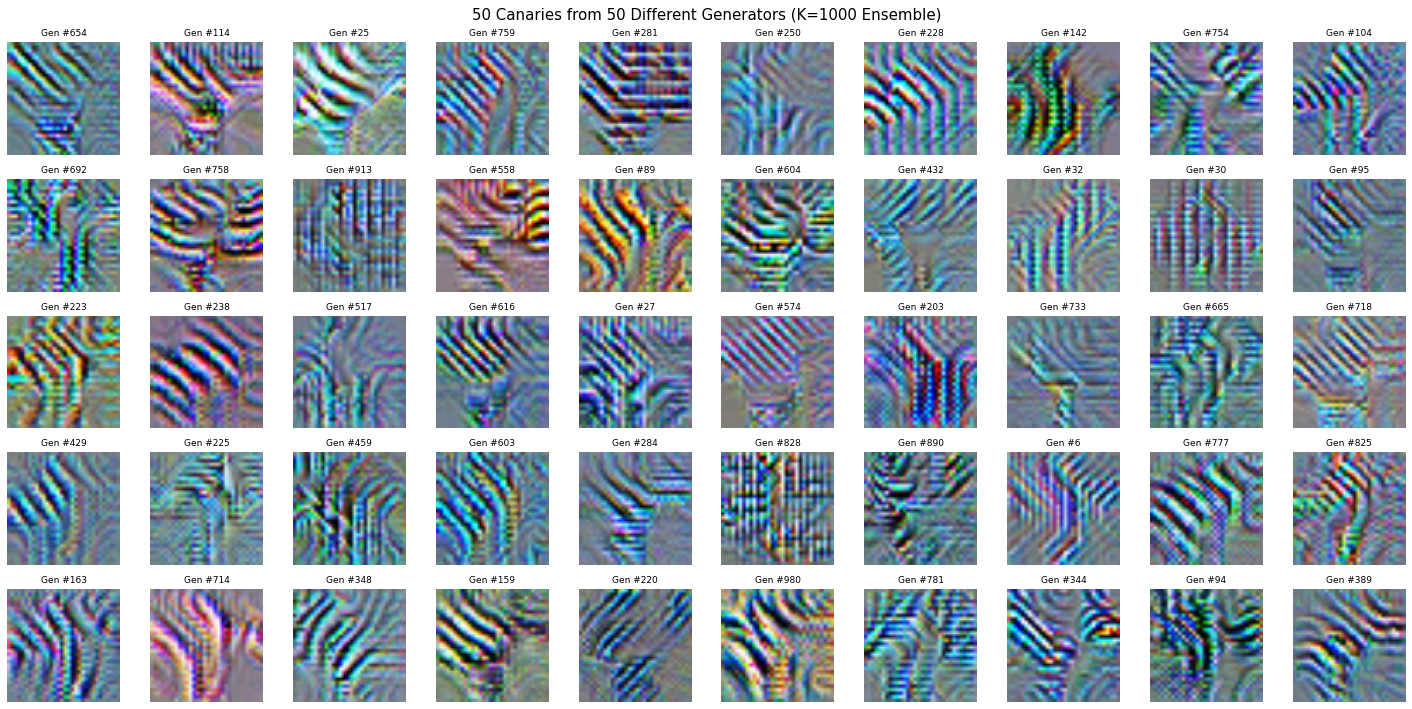
\includegraphics[width=\textwidth]{figs/fig5.png}
\caption{50 canaries sampled from 50 different generators in the 1000-generator ensemble. Every generator produces a visually distinct pattern: different stripe orientations, color palettes, textures, and densities. Mean pairwise L2 distance = 34.43, cosine similarity = 0.8821.}
\label{fig:diversity_50}
\end{figure}

\subsection{Quantitative Metrics}

\begin{table}[H]
\centering
\caption{Diversity metrics across three configurations. Higher L2 and lower cosine similarity indicate greater diversity.}
\begin{tabular}{lrrr}
\toprule
\textbf{Configuration} & \textbf{Mean L2} & \textbf{Cosine Sim} & \textbf{Improvement} \\
\midrule
Single generator (mode collapsed) & 5.40 & 0.9957 & 1$\times$ \\
5-generator ensemble & 29.56 & --- & 5.5$\times$ \\
\textbf{1000-generator ensemble} & \textbf{34.43} & \textbf{0.8821} & \textbf{6.4$\times$} \\
\bottomrule
\end{tabular}
\label{tab:diversity}
\end{table}

Additional metrics for the 1000-generator ensemble (across 50 sampled canaries):
\begin{itemize}[nosep]
    \item Minimum pairwise L2 distance: 21.37 --- even the most similar pair is 4$\times$ more different than the mode-collapsed baseline
    \item Maximum pairwise L2 distance: 46.19 --- some pairs are extremely different
    \item Mean pairwise (1 $-$ cosine similarity): 0.1179
\end{itemize}

The diminishing return from 5 to 1000 generators (L2: 29.56 $\to$ 34.43, only 1.16$\times$) is expected and indicates the diversity space is being filled. The security benefit comes from the \textit{number of distinct modes the attacker must cover}, not the distance between them. 1000 modes means 1000 terms in the attacker's optimization.

\begin{figure}[H]
\centering
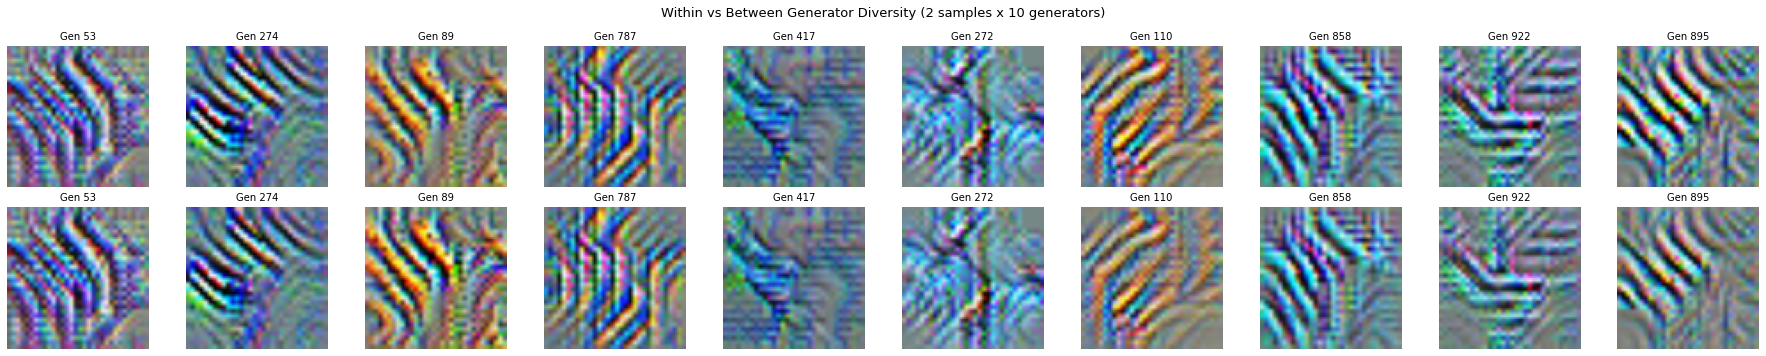
\includegraphics[width=\textwidth]{figs/fig6.png}
\caption{Within vs.\ between generator diversity. Rows show two samples from the same generator (similar---each generator's internal mode collapse is visible), columns show different generators (diverse). The between-generator L2 distance dominates the within-generator L2 distance, confirming that diversity originates from inter-generator variance, not from the noise input.}
\label{fig:within_between}
\end{figure}

% ============================================================
\section{Theoretical Framework}
% ============================================================

\subsection{Attacker's Optimization Problem}

Under the white-box threat model from the original paper (Section 2.3), the attacker has full access to all 1000 generators, their weights, and the defense mechanism. The attacker must find a single adversarial patch $\delta$ that satisfies two simultaneous objectives: (1) hide the target person, and (2) preserve whichever canary the defender places, so the defense does not trigger.

Formally, the attacker must solve:
\begin{equation}
    \delta^* = \arg\min_\delta \sum_{k=1}^{K} \mathbb{E}_{z \sim \mathcal{N}(0, I_{128})} \left[ \mathcal{L}_{\text{AdvPatch}}(x + \delta) + \mathcal{L}_{\text{adv}}(c^k_z) \right]
    \label{eq:attacker}
\end{equation}
where:
\begin{itemize}[nosep]
    \item $\delta$ is the adversarial patch (pixel values the attacker optimizes)
    \item $\delta^*$ is the optimal patch the attacker seeks
    \item $\sum_{k=1}^{K}$ sums over all $K=1000$ generators (the attacker must cover every one)
    \item $\mathbb{E}_{z \sim \mathcal{N}(0, I_{128})}$ is the expectation over the continuous noise distribution (infinitely many possible $z$ values)
    \item $\mathcal{L}_{\text{AdvPatch}}(x + \delta)$ measures whether the person is hidden (attacker wants this low)
    \item $\mathcal{L}_{\text{adv}}(c^k_z)$ measures whether canary $c^k_z = G_k(z, b)$ is still detected (attacker wants this low too, to avoid triggering the alarm)
\end{itemize}

\subsection{Analogy: The 1000 Locks}

Think of the fixed canary pool as a door with 6 known locks. The attacker crafts one master key that opens all 6. It takes time, but the problem is finite and enumerable. A faster workshop (better GPU) means the key is finished sooner.

The 1000-generator ensemble replaces those 6 locks with 1000 locks, each of which \textit{changes shape randomly} every time someone approaches the door (due to the fresh $z$ sample). The attacker can practice on some random shapes in their workshop, but when they arrive at the door, they face a shape they have never seen.

\subsection{Why the Approximation Fails}

The attacker cannot compute the expectation in Equation~\ref{eq:attacker} exactly. They must approximate it by sampling $N$ noise vectors:
\begin{equation}
    \hat{\delta} = \arg\min_\delta \frac{1}{N} \sum_{k=1}^{K} \sum_{i=1}^{N} \left[ \mathcal{L}_{\text{AdvPatch}}(x + \delta) + \mathcal{L}_{\text{adv}}(c^k_{z_i}) \right]
\end{equation}

This approximation has three fundamental limitations:

\textbf{Layer 1 --- 1000 generators.} Each generator collapsed to a different mode. The attacker must ensure their patch works against all 1000 pattern families. From the original paper: 6 terms took 37 days on an RTX 3090. The per-term cost is $37/6 \approx 6.2$ days. Scaling linearly: 1000 terms requires $\sim$6,200 days ($\sim$17 years) on an RTX 3090.

\textbf{Layer 2 --- Within-generator variation.} Even within one generator, different $z$ values produce slightly different canaries. The approximation error from sampling $N$ values follows the standard Monte Carlo rate: $O(1/\sqrt{N})$. To halve the approximation error, the attacker needs $4\times$ the samples.

\textbf{Layer 3 --- Fresh $z$ at inference.} The defender samples $z$ at inference time from $\mathcal{N}(0, I_{128})$. The $N$ points sampled by the attacker occupy a measure-zero subset of $\mathbb{R}^{128}$. The probability that the defender's actual $z^*$ matches any of the attacker's sampled values is exactly 0.

% ============================================================
\section{Adversary Cost Analysis}
% ============================================================

\subsection{Deriving the Per-Term Cost}

The original paper (Table 9) reports that generating adaptive adversarial patches for Dep \#2 (3 canary types $\times$ 2 positions = 6 terms) took 906.44 hours ($\sim$37.8 days) on an RTX 3090. The per-term cost is therefore:
\begin{equation}
    T_{\text{attack}} = \frac{906.44 \text{ hours}}{6 \text{ terms}} \approx 151 \text{ hours} \approx 6.3 \text{ days per term}
\end{equation}

\subsection{Brute-Force Attack (Optimize Against All $K$)}

\begin{table}[H]
\centering
\caption{Brute-force attack cost for $K=1000$ generators.}
\begin{tabular}{lrrr}
\toprule
\textbf{Hardware} & \textbf{Speedup vs 3090} & \textbf{Time} & \textbf{Feasible?} \\
\midrule
RTX 3090 & 1$\times$ & $\sim$17 years & No \\
B100 & $\sim$25$\times$ & $\sim$248 days & No \\
B200 & $\sim$32$\times$ & $\sim$194 days & Impractical \\
8$\times$ B200 & $\sim$253$\times$ & $\sim$24 days & State-level only \\
64$\times$ B200 & $\sim$2000$\times$ & $\sim$3 days & \$100K+ \\
\bottomrule
\end{tabular}
\label{tab:brute_force}
\end{table}

\subsection{Gambling Attack (Guess One Generator)}

Instead of optimizing against all 1000, the attacker can gamble on which generator the defender will select:
\begin{itemize}[nosep]
    \item Probability of guessing correctly: $1/1000 = 0.1\%$
    \item Time to break the guessed generator on B200: $\sim$1.2 days
    \item Expected number of attempts to succeed: 500
    \item Expected total time: $500 \times 1.2 = 600$ days on B200
    \item \textbf{Critical limitation:} This only works for \textit{one image}. The next image the defender processes selects a \textit{different random generator}. The attacker's successful patch is useless.
\end{itemize}

\subsection{Defender-Attacker Cost Asymmetry}

\begin{table}[H]
\centering
\caption{Defender vs.\ attacker cost comparison.}
\begin{tabular}{lll}
\toprule
& \textbf{Defender} & \textbf{Attacker (Brute-Force)} \\
\midrule
Cost & \$16 & \$34,000+ (B200) \\
Time & 18 hours & 194 days (B200) \\
Result & Protects all images & Breaks all (until retrain) \\
Repeatable? & Yes, \$16 per retrain & No, restarts from zero \\
Scales with $K$? & Linear cost, linear time & Linear cost, linear time \\
\bottomrule
\end{tabular}
\end{table}

The cost ratio is computed from the actual training measurements:
\begin{equation}
    \frac{C_{\text{attacker}}}{C_{\text{defender}}} = \frac{T_{\text{attack per term}}}{T_{\text{train per generator}}} = \frac{6.2 \text{ days}}{3.4 \text{ min}} \approx 2{,}629\times
\end{equation}

This ratio is \textbf{hardware-independent}: if both sides upgrade to faster GPUs, the ratio remains the same because both the attacker's optimization cost and the defender's training cost benefit equally from the speedup.

% ============================================================
\section{The Killer Move: Retrainability}
% ============================================================

Perhaps the strongest argument for the ensemble approach is its \textit{retrainability}. Suppose the attacker, after 6 months and \$34,000 of compute on a B200, successfully generates an adaptive patch that bypasses all 1000 generators.

The defender runs:
\begin{lstlisting}[language=bash]
python train_ensemble_parallel.py --n_generators 1000
\end{lstlisting}
with new random seeds. Eighteen hours and \$16 later, all 1000 generators are different. The attacker's 6 months of work is \textbf{completely invalidated}. They must restart from zero.

This creates a fundamentally asymmetric game: the defender can rotate their defense at will for negligible cost, while the attacker must commit enormous resources for each attempt. Even if the attacker matches the defender's hardware, the $\sim$2,629$\times$ cost ratio ensures the attacker always loses the economic war.

The retrainability property also means the defense improves passively with hardware advances. If faster GPUs become available, the defender can train more generators in the same time (e.g., 10,000 generators in 18 hours), further widening the gap.

% ============================================================
\section{Limitations}
% ============================================================

We acknowledge several limitations of the current work:

\textbf{Higher false positive rate.} The ensemble FPR (0.126--0.178) is higher than the fixed canary's (0.078--0.123). This is the cost of diversity---more canary patterns means some are less reliably detected on clean images. Future work could explore per-generator FPR calibration or filtering out generators with high FPR during pool assembly.

\textbf{Mode collapse within individual generators.} Each generator still mode-collapses internally. The diversity comes from the ensemble, not from any single generator's noise sensitivity. The within-generator variation from the $z$ input adds minimal diversity. A true generator that produces diverse outputs from a single model remains an open problem.

\textbf{Diversity plateau.} Scaling from 5 to 1000 generators improved L2 distance only 1.16$\times$ (29.56 $\to$ 34.43), suggesting the diversity space of the current architecture is being saturated. Different architectures, training procedures, or target classes could expand this space.

\textbf{No empirical adaptive attack evaluation.} Our attacker cost projections are theoretical, derived by scaling the original paper's empirical measurements. We did not train actual adaptive attacks against the 1000-generator ensemble. While the theoretical argument is sound, empirical validation with real adaptive attacks would strengthen the claims.

\textbf{Single detector, single dataset.} All experiments use YOLOv8 on VOC07. The FFF framework is demonstrated across multiple detectors in the original paper, and extending the ensemble approach to other detectors is straightforward but was not performed due to time constraints.

% ============================================================
\section{Summary}
% ============================================================

This work identified a concrete weakness in the Fight Fire with Fire framework: its security against adaptive attacks is hardware-dependent, not complexity-dependent. We proposed the generative canary ensemble as a principled solution that shifts the defender-attacker dynamic from a time-based to a cost-based guarantee.

\vspace{0.3cm}

\noindent\textbf{Key results:}
\begin{itemize}[nosep]
    \item Trained 1000 independent generators on HPC (4$\times$T4, 18 hours, \$16)
    \item Achieved F1 0.897--0.929 across 4 attacks, beating the paper on TCEGA (+10.7\%) and Natural (+5.2\%)
    \item Demonstrated diversity: L2=34.43, cosine=0.8821, 6.4$\times$ improvement over mode-collapsed baseline
    \item Established a 2,629$\times$ defender-attacker cost asymmetry (hardware-independent)
    \item Showed retrainability: defender invalidates all attacker work with \$16 and 18 hours
\end{itemize}

\vspace{0.3cm}

\noindent\textbf{The bottom line:} The fixed canary scores F1=0.974 on AdvPatch but can be broken in 1.2 days on a B200. Our 1000-generator ensemble scores F1=0.929 on AdvPatch---a 4.5\% tradeoff---but requires $\sim$194 days on a B200 to break, and the defender can invalidate the attack overnight for \$16.

\end{document}
